\documentclass[10pt,a4paper]{article}

\usepackage[utf8]{inputenc}
\usepackage{amsmath}
\usepackage{amsfonts}
\usepackage{amssymb}
\usepackage{tikz}
\usepackage{pgf}
\usetikzlibrary{arrows,automata}

\title{Implementation and evaluation of model checking using modal mu-calculus}

\author{Olav Bunte (0803961), Maurice Laveaux (0813568),\\ Ziad Ben Snaiba (0748095)}

\date{\today}

\begin{document}
\maketitle

\section{Introduction}
This report elaborates on our work and findings of assignment on, which is split in two parts. The first part of the assignment is to implement two versions of the model checking algorithm for modal mu-calculus: a naive version and the Emerson-Lei version. The second part is to evaluate these two versions using provided testcases supplemented with modal mu-calculus formulas of our own.\\
In section \ref{design} we will explain our design of the algorithm. The testcases and their result when used on the algorithm is shown in section 3. Lastly, we conclude this report in section 4.

\section{Design}
\label{design}
In this section the design of our model checking algorithm is given, which we have coded in C++. First we will show the data structure of modal mu-calculus formulas and how they are constructed. Then we elaborate on the design of the solving algorithm divided in what the two versions of the algorithm have in common and what is special to each version.

% data structure of formula, parsing
\subsection{Modal mu-calculus formulas}
Since the modal mu-calculus is defined recursively, we have decided to store mu-calculus formulas the same way. To do so we've implemented a class \texttt{MuFormula}, which represent a subformula of the given mu-calculus formula. This \texttt{MuFormula} can hold up to two pointers two other subformulas, which are its direct subformulas. These subformulas combined by an operation form the \texttt{MuFormula}, as it is defined in the modal mu-calculus grammar. This operation is implemented as the enum \texttt{Op} which can have the following values:
\begin{itemize}
\item FALSE: the value false
\item TRUE: the value true
\item VAR: a variable
\item AND: logical and
\item OR: logical or
\item DIAMOND: the diamond operator
\item BOX: the box operator
\item MU: the least fixed point operator
\item NU: the greatest fixed point operator
\end{itemize}
When $\texttt{Op} \in \{\text{FALSE}, \text{TRUE}, \text{VAR}\}$ no subformula is defined, when $\texttt{Op} \in \{\text{AND}, \text{OR}\}$ both subformulas are defined and else only the first subformula is defined.\\
For the cases $\texttt{Op} \in \{\text{BOX}, \text{DIAMOND}\}$ the \texttt{MuFormula} needs to know the transition label and for the cases $\texttt{Op} \in \{\text{VAR}, \text{MU}, \text{NU}\}$ the \texttt{MuFormula} needs to know the name of the variable. These labels and variable names are stored as a string. Since these cases are distinct, we have decided to store these values in the same string variable, named \texttt{varlabel}, to reduce memory usage.



% basis (solve method), what naive and EL have in common
\subsection{Solving algorithm}


% what is special to naive
\subsubsection{Naive algorithm}


% what is special to EL
\subsubsection{Emerson-Lei algorithm}


\section{Evaluation}

\input{dining}

\input{demanding}

\input{boardgame}

\section{Conclusion}


A picture of the labelled transition system.

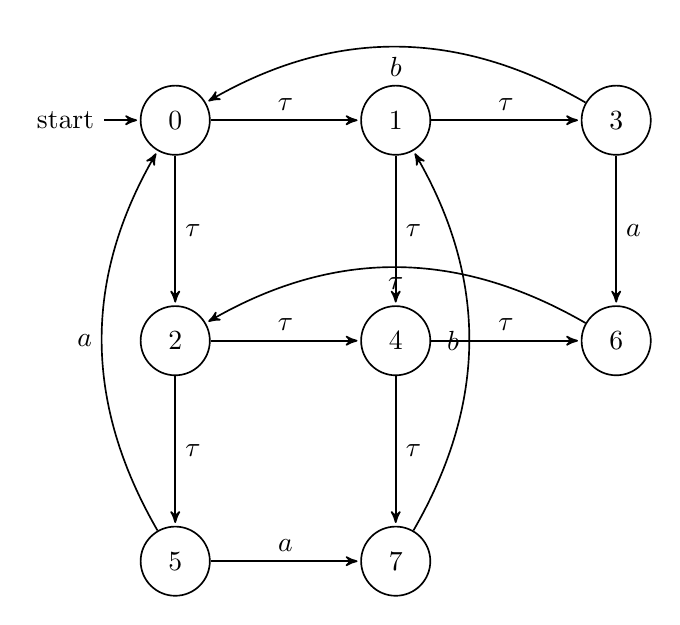
\begin{tikzpicture}[->,>=stealth', shorten >=1pt,auto, node distance=2.8cm, semithick]
  \tikzstyle{every state}=[text=black]

  \node[initial,state] (0)                    {$0$};
  \node[state]         (1) [right of=0] {$1$};
  \node[state]         (2) [below of=0] {$2$};
  \node[state]         (3) [right of=1] {$3$};
  \node[state]         (4) [below of=1] {$4$};
  \node[state]         (5) [below of=2] {$5$};
  \node[state]         (6) [right of=4] {$6$};
  \node[state]         (7) [below of=4] {$7$};
  
 \path (0) edge node {$\tau$} (1)
 	   (0) edge node {$\tau$} (2)
 	   (1) edge node {$\tau$} (3)
 	   (1) edge node {$\tau$} (4)
 	   (2) edge node {$\tau$} (5)
 	   (2) edge node {$\tau$} (4)
 	   (3) edge node {$a$} 	  (6)
 	   (3) edge [bend right] node {$b$} 	  (0)
 	   (4) edge node {$\tau$} (6)
 	   (4) edge node {$\tau$} (7)
 	   (5) edge [bend left] node {$a$}    (0)
 	   (5) edge node {$a$}    (7)
 	   (6) edge [bend right] node {$\tau$} (2)
 	   (7) edge [bend right] node {$b$}    (1);
\end{tikzpicture}

\end{document}